% !TeX encoding = UTF-8
% !TeX spellcheck = es_ES
% !TeX root = Esquema.tex
% !TEX root = Esquema.tex

\section{Zonas de la maqueta}
El diseño esta basado en la versiones AE y ABC de piko, el nucleo central es la AE, añadiendo una estacion interna y una playa de vias externa. Insipirado en ABC

\begin{figure}[H]
    \centering
	\includegraphics[scale=.25]{Imagenes/PikoAE.png}
   \includegraphics[scale=.25]{Imagenes/PikoABC.png}
    \caption{Inspiracion Original}
    \label{fig:PikoOrigen}
\end{figure}

Asi pues, Daniel Bahn esta organizada 4 Zonas:
\begin{itemize}
\item Linea principal, en negro
\item Estacion, en rojo 
\item Estacion termino, en Verde
\item Playa de vias o Yard, en cyan

\end{itemize}
\begin{figure}[H]
    \centering
\begin{tikzpicture}

    %\draw [very thin, green]  (-6,-3) grid (6,3);
	\paintBoard 
	\paintStation[red]{2pt}
    \paintTerminus[green]{2pt}
    \paintYard[cyan]{2pt}
	\paintMain[black]{4pt}

\end{tikzpicture}

    \caption{Zonas de la maqueta}
    \label{fig:ZonasMaqueta}
\end{figure}

\subsection{Version Lineal}
Para entender la maqueta pongamosla en una version lineal. Para ello empezarmos antes de la playa de vias y seguiremos la norma de circulacion Oeste a Este\sidenote{Norte en el centro de la maqueta, lo que conlleva un sentido contrario a las agujas del reloj}

\begin{figure}[H]
    \centering
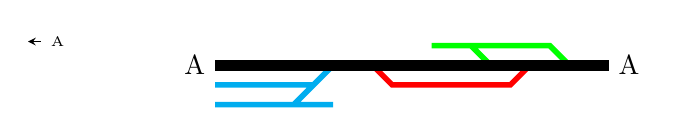
\begin{tikzpicture}
    \begin{scope}[scale=0.25,shift={(-8,0)}]
        \paintBoard 
        \paintStation[red]{0.5pt}
        \paintTerminus[green]{0.5pt}
        \paintYard[cyan]{0.5pt}         
        \paintMain[black]{1pt}
        \node[] (start) at (0,1.20) {\tiny A};
        \draw[line width=.25pt,-stealth] (start.west) -- (-1.5,1.20);
    \end{scope}
\node[left] at (0,0) {A};

\node[right] at (5,0) {A};

\draw[color=cyan, line width=2pt] (0,-0.5) -- (1.5,-0.5) (1,-.5) -- (1.5,0) (0,-0.25)--(1.25,-0.25);
\draw[color=red,line width=2pt] (2,0)--(2.25,-0.25) -- (3.75,-0.25)--(4,0);

\draw[color=green,line width=2pt] (2.75,0.25)-- (4.25,0.25) -- (4.5,0)
(3.25,0.25) -- (3.5,0) ;
\draw[color=black, line width=4pt] (0,0) -- (5,0);
\end{tikzpicture}

\caption{Version Lineal}
    \label{fig:VersionLineal}
\end{figure}



\subsection{Extension Virtual}
Esta maqueta se puede extender de una manera ficticia, donde cada zona puede representar diferentes elementos de una red mas grande tras dar una serie vueltas por el ciclo principal.

\begin{figure}[H]
    \centering
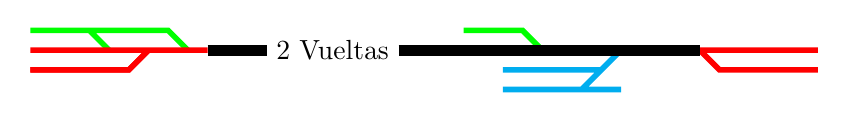
\begin{tikzpicture}

\draw[color=cyan, line width=2pt] (6,-0.5) -- (7.5,-0.5) (7,-.5) -- (7.5,0) (6,-0.25)--(7.25,-0.25);

\draw[color=green,line width=2pt] (0,0.25)-- (1.75,0.25) -- (2,0)
(0.75,0.25) -- (1,0) ;

\draw[color=red,line width=2pt](0,-0.25) -- (1.25,-0.25)--(1.5,0) (0,0)--(2.25,0);
\draw[color=red,line width=2pt](0,-0.25) -- (1.25,-0.25)--(1.5,0);
\draw[color=black, line width=4pt] (2.25,0) -- (3,0); 
\node[right](txt) at (3,0) {2 Vueltas};

\draw [color=green,line width=2pt] (5.5,0.25)-- (6.25,0.25) -- (6.5,0);

\draw[color=red,line width=2pt](8.5,0) -- (8.75,-0.25)--(10,-0.25) (8.5,0)--(10,0);


\draw[color=black, line width=4pt] (txt.east) -- (8.5,0);

\end{tikzpicture}

\caption{Version Lineal Alargada}
    \label{fig:VersionLinealAlargada}
\end{figure}

En este caso, hemos creado dos estaciones termino, empezamos en la zona <<estacion>> y <<estacion termino>>. Una vez que salimos de la estacion daremos dos vueltas a la via principal.Durante estas dos vueltas ignoraremos los desvios de las zonas <<playa de vias>> y <<estacion termino>>. Pero una vez que hemos dado las dos vueltas la zona <<estacion termino>> repesentara en este caso una linea industrial y justo despues ya tenemos la playa de vias y la estacion final.

No obstante, se documentaran diferentes escenarios en futuros documentos.

